\section{Optimizador y Algoritmo Genético}
%
% Se seleccionó un algoritmo genético (AG) como método de optimización por ser un
% método sencillo de programar además, este tipo de algorimto es de utilidad
% cuando se tiene una solución con uno o más máximos óptimos locales ó cuando no
% se tiene certeza sobra la suavidad de la función a evaluar.
%

Se seleccionó un algoritmo genético para realizar la optimización de la
geometría del MRCVC por la simplicidad y facilidad de implementación del mismo.
%
Si bien este tipo de métodos no garantizan que se alcance un resultado óptimo,
en la práctica se ha observado que alcanzan soluciones muy cercanas a las
óptimas tras pocas iteraciones del método~\parencite{goldberg}\parencite{shi}.

Una de las ventajas de este método es que no requiere información del gradiente
de la función que se está evaluando, lo cual es útil cuando no se puede asegurar
la existencia de la derivada de la función en todo el dominio ó cuando se tiene
una función con más de un máximo o mínimo local.
%
Además, el punto de partida de la optimización es una población generada al
azar, de modo que se tiene un muestreo aleatorio del dominio que se está
evaluando.
%
Esto hace que el método sea poco susceptible a caer en un óptimo local.

Se puede decir que un algoritmo genético es un método de búsqueda aleatoria
guiada.
%
¿Cómo difieren los AG de los métodos tradicionales de búsqueda?
%
\begin{enumerate}
  \item Los AG pueden operar sobre una representación de las variables estudiadas y
no necesariamente sobre las variables de estudio.
  \item Cada iteración utiliza un conjunto de datos con cierto grado de
aleatoreidad..
  \item Utilizan una función objetivo para evaluar cada punto sin necesidad de
conocer la derivada de la función que se está evaluando.
  \item Los AG usan reglas probabilísticas, no deterministas.
\end{enumerate}

Otros métodos de optimización se mueven de un punto al siguiente en el espacio
solución, basándose en alguna regla de decisión lo que puede dar como resultado
un máximo (o mínimo) local.

\subsection{Componentes básicos de un AG}
%
Los mecanismos básicos que hacen a un algoritmo genético son: 1) SELECCIÓN,
2) CRUZA y 3) MUTACIÓN, el funcionamiento básico se sintetiza en el
pseudocódigo~\ref{algo:genetico}.

La SELECCIÓN consiste en crear individuos a partir del puntaje que devuelve
una función objetivo, la cual es la encargada de guiar el proceso de
optimización dando mayor o menor puntaje a un candidato según el resultado que
se quiere obtener.
%
Este paso significa que aquellos individuos a los cuales se les asignó un
puntaje más elevado tienen más probabilidades de ser copiados o ``transmitir''
sus parámetros a la iteración siguiente, este proceso imita en cierta forma la
selección natural o evolución Darwiniana y de aquí viene el nombre de algoritmo
genético o evolutivo.

El segundo operador es la CRUZA, consiste en combinar los parámetros de dos
individuos para obtener uno nuevo, esto se asemeja a la reproducción.

Finalmente la MUTACIÓN es la encargada de modificar aleatoriamente uno o más
parámetros de cada nuevo individuo.
%
Este operador juega un rol secundario pero muy importante, es secundario porque
se pueden alcanzar soluciones satisfactorias sin incluir este mecanismo sin
embargo, se utiliza con probabilidades pequeñas para evitar la pérdida temprana
de información relevante.
%
Si la probabilidad de mutación es muy alta, el AG se convierte en un algoritmo
de búsqueda aleatoria.


\begin{algorithm} \caption{Algoritmo de optimización}\label{algo:genetico}
  generación = 0;
  Inicializar población.\;
  \While{No se cumpla condición de parada}{
    SELECCIÓN se crean y seleccionan los individuos más aptos.\;
    CRUZA los candidatos seleccionados (creación de la anueva población)\;
    MUTACIÓN algunos individuos de la nueva población\;
    generación = generación + 1\;
    \If{Verifica condición de parada}{
      Parar\;
    }
  }
  {Guardar resultados\;}
\end{algorithm}

%
% \subsection{Implementación}
%
Gran parte de este trabajo fue utilizar a ICESym como parte de la función
objetivo aprovechando la cualidad de ``caja negra'' que se le puede dar al
simulador.
%
Para lograr esto se modificó parte del código de ICESym con el objetivo de
facilitar la configuración, ejecución y lectura de los resultados que arroja el
simulador y así poder ejecutar de manera automatica una simulación con una
configuración particular del motor.
%
Otro aspecto del optimizador que se desarrolló es el de poder ejecutar múltiples
instancias de ICESym en paralelo para reducir el tiempo de ejecución cada
simulación, pudiendo evaluar varios motores (o individuos) al mismo tiempo.

Para la primer iteración se programaron desde cero los algoritmos y funciones
necesarias para llevar a cabo la optimización,  posteriormente se tomo la la
librería DEAP~\parencite{DEAP_JMLR2012} y se modificaron los operadores a medida,
para poder utilizarlos con ICESym.

En los apartados siguientes se describe la implementación de cada uno de los
operadores en el optimizador.

\subsection{Población}
%
Se decidió representar cada motor como un vector con las dimensiones y reglaje
que definen la geometría del sistema de intercambio de gases, los cuales se
listan en la tabla~\ref{tab:param_motor}.
%
Se limitó los valores que puede tomar cada parámetro para que la geometría
resultante se asemeje a la geometría del motor utilizado en trabajos anteriores.


\begin{table}[ht]
  \centering
  \begin{tabular}{rllll} \toprule
    Nº & Parámetro & Descripción & Sistema & Límites \\ \midrule
    1 & DTA & Diámetro de tubo & Admisión & [60, 100] mm \\
    2 & DTE & Diámetro de tubo & Escape & [60, 100] mm\\
    3 & LIT & Largo de tubo & Admisión & [300, 2000] mm\\
    4 & LET & Largo de tubo & Escape & [300, 2000] mm\\
    5 & IIA & Ángulo de apertura & Admisión & [0,90]º \\
    6 & IFA & Ángulo geométrico de cierre & Admisión & [IIA, 90]º \\
    7 & IIE & Ángulo geométrico de apertura & Escape & [0, 90]º \\
    8 & IFE & Ángulo geométrico de cierre & Escape & [IIA, 90]º \\ \bottomrule
  \end{tabular}
  \caption{Parámetros que representan al motor}\label{tab:param_motor}
\end{table}


Se decidió representar los vectores que hacen a cada motor como un número
binario de 40 dígitos, ocupando 5 dígitos para representar cada uno de los 8
parámetros que hacen a cada motor.
%
Esto facilita la implementación de los operadores de selección, cruza y
mutación, pudiendo aprovechar implementaciones de operadores existentes en
librerías como DEAP.
%
Estos 8 números binarios luego se convierten una lista de enteros que mediante
un cambio de escala $f(x)$, en la que se ingresa con un entero entre 0 y
$2^{n}-1$, siendo $n$ la cantidad de dígitos del binario (en este caso 5).
%
Los coeficientes $a$ y $b$ son tal que $f(0)=x_{0}$ y $f(2^{n}-1) = x_{1}$,
donde $x_{0}$ y $x_{1}$ son los extremos del rango para el que se quiere aplicar
la transformación.
%
Los coeficientes $a$ y $b$ son particulares a cada parámetro, porque se
determinan de acuerdo a los valores que puede tomar cada uno.

De este modo se obtienen el valor de cada uno de los parámetros que hacen a la
configuración particular de cada motor en ICESym, ver figura~\ref{fig:pop_bit}.
%
El orden de los mismos se mantiene constante, por lo que cada sección del número
representa una característica en particular del motor.
%

\begin{figure}[ht]
  \centering
  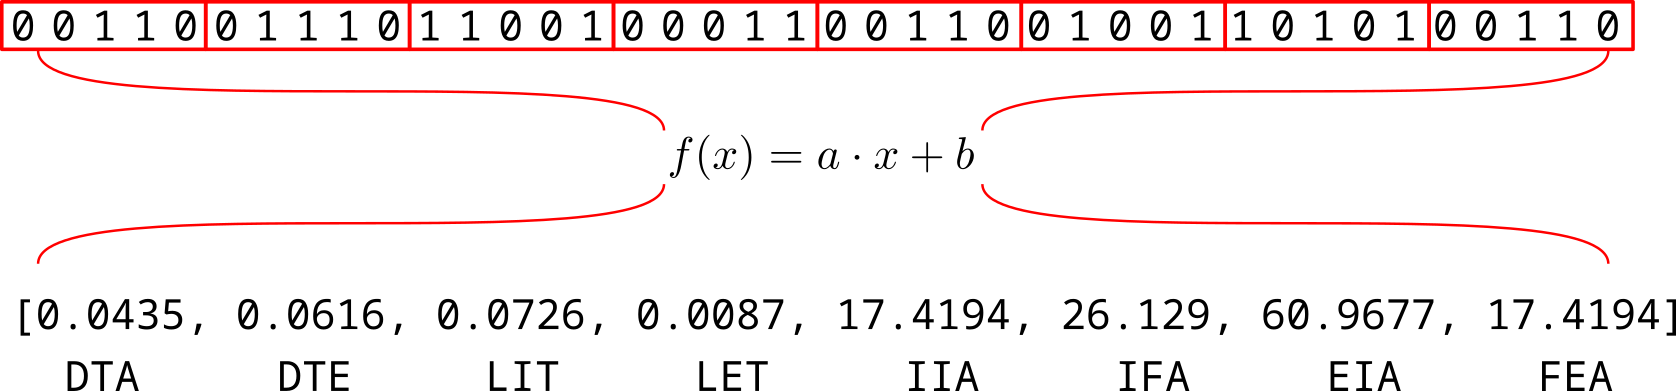
\includegraphics[]{genetico/representacion_bits.png}
  \caption{Individuo como binario}\label{fig:pop_bit}
\end{figure}


\subsection{Reproducción}

Para crear la nueva población se debe elegir a los nuevos candidatos basándose
en los puntajes de la población actual, hay varios métodos diferentes de
selección, como son de ruleta, aleatoria, por puntaje y de tipo torneo.
%
El método seleccionado es el torneo, el cual consiste en comparar los puntajes
de $n$ individuos seleccionados al azar y el que tenga el mejor puntaje es el
seleccioando o ganador.
%
La cantidad de individuos comparados $n$ es el tamaño de muestreo o de torneo,
cuanto más grande sea este número más posibilidades tiene de ganar los
individuos con mayor puntaje y la cantidad de rondas del torneo determina la
cantidad de individuos seleccionados para participar en la próxima iteración o
generación de candidatos.


\subsection{Cruza}
%
El operador de cruza se encarga de combinar los genes de dos individuos para
producir un individuo nuevo, la función es la de intercambiar los parámetros que
hacen a uno y otro para dar lugar a una nueva posible solución
%
Para individuos representados por un vector se suelen usar operadores de tipo
curza de uno o mùltiples puntos como tambièn cruza uniforme.
%
El método seleccionado es \emph{cruza de dos puntos}, en este método
se corta el vector que forma al individuo en dos puntos, la posición de estos
puntos se selecciona al azar, manteniendo el largo original de los vectores.
%
Luego los individuos ``cruzados'' se combinan de forma complementaria, como en
la figura~\ref{fig:cr2puntos}, en el algoritmo~\ref{algo:cr2puntos} se esquematiza
el proceso.
% TODO: pongo pseudocódigo? o dejo el còdigo

\begin{figure}
  \centering
  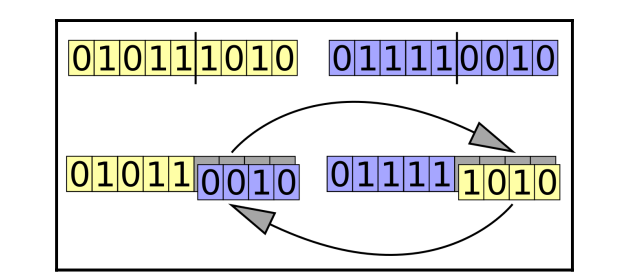
\includegraphics[width=0.5\textwidth]{cruza2puntos.png}
  \caption{Cruza de dos puntos}\label{fig:cr2puntos}
\end{figure}


\begin{algorithm}[]
  \KwIn{\\
    $ind_{1}, ind_{2}$: dos individuos de entrada [101\ldots011], [110\ldots100]\\
    EA(a, b): devuelve un Entero al Azar entre los enteros a y b.\\
    L(a): devuelve la cantidad de elementos en a.}
  \KwOut{\\
    $ind_{1}, ind_{2}$: individuos de entrada modificados}
  \SetKwFunction{EA}{EA}
  \SetKwFunction{L}{L}
  % \SetKwFunction{min}{min}
  \BlankLine
  s = min(\L{$ind_{1}$}, \L {$ind_{2}$})\;
  $CX_{1} = \EA{1, s}$\;
  $CX_{2} = \EA{1, s-1}$\;
  \eIf{$CX_{1} \geq CX_{2}$}{
    $CX_{2} = CX_{2}+1$\;
  }{
    $aux=CX_{1}$\;
    $CX_{1}=CX_{2}$\;
    $CX_{2}=aux$\;
  }
  $aux = ind_{1}$\;
  $ind_{1}[CX_{1}:CX_{2}] = ind_{2}[CX_{1}:CX_{2}]$\;
  $ind_{2}[CX_{1}:CX_{2}] = aux[CX_{1}:CX_{2}]$\;
  \Return{$ind_{1}, ind_{2}$}\;
  Terminar el programa;
  \caption{Cruza de dos puntos}\label{algo:cr2puntos}
\end{algorithm}

\subsection{Mutación}
%
La mutación juega un rol secundario pero importante, una pequeña probabilidad
de que alguno de los genes se modifique en un valor aleatorio contribuye a que
el algoritmo genético no se estanque en soluciones máximos o mínimos locales.

Algunos de los métodos de mutación utilizados son: 1) FLIP BIT, 2) INTERCAMBIO,
3) INVERSION, 4) REORDENADO ALEATORIO.

% FLIP BIT se utiliza para números binarios y el método consiste en intercambiar
% ceros y unos con una probabilidad al azar en ubicaciones al azar, por ejemplo
% $10101 \rightarrow 11101$.

para este método se cambian al azar el orden de los números que hacen al
individuo, modificando la lista, por ejemplo: $12345 \rightarrow 12543$.

\subsection{Función objetivo}\label{sec:funcion_objetivo}
%
La función objetivo es la encargada de dar puntaje a los individuos, en la
analogía con la selección natural esta función es el ambiente, la que determina
que tan bien se desempeña un motor con respecto a otro en lo que respecta
\emph{performance} del sistema de intercambio de gases.
%
Inicialmente se propuso que la función objetivo sea la suma de los rendimientos
volumétricos a todas las velocidades simuladas, este tipo de funciones da como
resultado una curva de rendimiento volumétrico aserrada como se muestra en la
figura~\ref{fig:curva_aserrada}

\begin{figure}[ht]
  \centering
  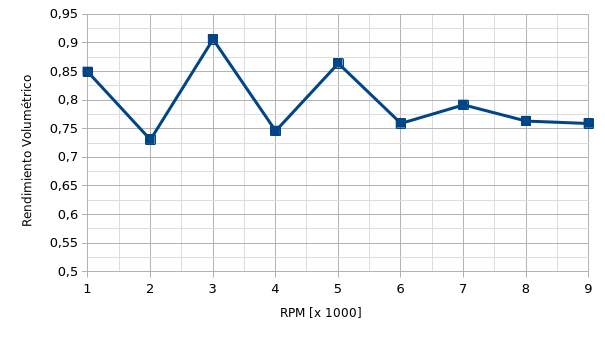
\includegraphics[width=0.7\textwidth]{genetico/curvas_aserradas.png}
  \caption{Curvas de rendimiento volumétrico aserradas}\label{fig:curva_aserrada}
\end{figure}


Este comportamiento aserrado es poco deseable, por lo que se modificó la
función para conseguir una curva de rendimiento volumétrico suave.
%
Además se implementó una suma ponderada, para obtener un rendimiento
volumétrico máximo en un valor arbitrario de 5000 RPM.\@
%
Para prevenir el comportamiento aserrado se introdujo un sistema de penalidades,
que resta puntaje si la derivada de la función se modifica de una velocidad a
otra.

Finalmente se optó por una sencilla suma del rendimiento volumétrico y la
fracción de gases residuales para 6000 RPM, esto provó ser la función objetivo
que mejores resultados dió, el código utilizado se lista a continuación.

% \begin{lstlisting}[float,label=lst:label,caption=falta]
% def local_evaluate_engine(individual):
%     """Takes a global instance of motor.MRCVC and calculates it's score based on
%     volumetric efficiency curve.
%     """
%     eng = utils.map_to_engine(individual, BINNARY_LEN,
%                               d_coeff, l_coeff, a_coeff)
%     if not m.check_angles(eng):
%         return False
%     config = m.list_to_config(eng)
%     counter = 0
%     run_flag = False
%     kargs, cyl_data, extras_data = m.run_and_read(
%         ENGINE_OBJ, config, multi=CORES)
%     vol_eff = m.calc_volumetric_efficiency(kargs, extras_data)
%     xr = m.calc_residual_gas_fraction(kargs, extras_data)

%     m.clean_files(ENGINE_OBJ)
%     if 0 in vol_eff:
%         return False
%     else:
%         # aux = [r+1/x for r, x in zip(vol_eff, xr)]
%         aux = [1/i for i in xr]
%         return aux
% \end{lstlisting}

\begin{algorithm} \caption{Evaluación del motor}\label{algo:pre_puntaje}
  \KwIn{\\
    $ind$, vector con parámetros del motor a evaluar.\\
  }
  \KwOut{\\
  $S$, un valor utilizado para calcular el puntaje del individuo.}
  \SetKwFunction{me}{transformar_a_motor}
  \SetKwFunction{lc}{lista}
  \BlankLine

  puntaje = 0\;
  Configurar simulación, $sim=f(ind)$\;
  Ejecutar y leer el simulador\;
  $\eta_{v}$ = Calcular el rendimeinto volumétrico\;
  $x_{r}$ = Calcular la fracción de gases residuales\;
  N = \L{$\eta_{v}$}
  \eIf{hay un cero en $\eta_{v}$
  }{$S=0$\;
  }{\For{i = 0 \KwTo N
    }{
      $S = S + \eta_{v,i}+ 1 \mathbini{/} x_{r,i}$\;
    }
  }
  \Return{$S$}\;
\end{algorithm}


\begin{algorithm} \caption{Función Objetivo}\label{algo:funcion_objetivo}
  \KwIn{\\
    $ind$, vector con parámetros del motor a evaluar.\\
    $idx$, índice del elemento del puntaje que se quiere ponderar.\\
  }
  \KwOut{\\
    $S^{*}$, }
  \SetKwFunction{evalEng}{evaluarMotor}
  \BlankLine

  $S = \evalEng{ind}$\;
  \eIf{
    $S^{*} \neq \emptyset$\;
  }{
    $S^{*} = \sum{S}$ + $S_{idx}^{2}$\;
  }{
    $S^{*}=1$\;
  }
  \Return{$S^{*}$}\;
\end{algorithm}


Durante las primeras iteraciones del método, las poblaciones iniciales contienen
una gran cantidad de geometrías inválidas que devuelven valores de puntaje 0, en
caso de que alguna de las soluciones tenga un puntaje relativamente alto, existe
la posibilidad de caer en una dominancia temprana de la población causando una
convergencia temprana.
%
Para evitar esto se usa unca un cambio de escala de los puntajes de todos los
individuos, algunos de los métodos utilizados son: transformación lineal,
truncado $\sigma$ y transformación exponencial.
%
En este trabajo se utilizará el escalado por transformación lineal, como se
indica en los algoritmos que siguen abajo.

\begin{algorithm} \caption{Algoritmo de pre-escalado}\label{algo:pre-escala}
  \KwIn{\\
    $F$, es un vector que contiene los puntajes de todos los individuos\;\\
    $k$, es un multiplicador para el escalado, se suele usar $f\in[1.2, 2]$\parencite{goldberg}\;\\
  }
  \KwOut{\\
    $a, b$, son los coeficientes para la transformación lineal $f(x)=a\cdot x + b$\;
  }
  \SetKwFunction{max}{max}
  \SetKwFunction{min}{min}
  \SetKwFunction{media}{media}
  \BlankLine

  $u_{max} = \max{F}$\;
  $u_{min} = \min{F}$\;
  $u_{medio} = \media{F}$\;
  $aux = (k\cdot u_{medio} - u_{max}) \mathbin{/} k-1$\;
  \eIf{$u_{min}> aux$}{
    $\Delta u = u_{max}-u_{avg}$\;
    $a = (k - 1) \cdot u_{avg} / \Delta u$\;
    $b = u_{avg} \cdot (u_{max} - k \cdot u_{avg}) /Delta u$\;
  }{
    \If{$\Delta \neq 0$}{
      $a = u_{avg} \mathbin{/} \Delta u$\;
      $b = -u_{min} \cdot u_{avg} \mathbin{/} \Delta u$ \;
    }{
      $a=1$\;
      $b=0$\;
    }
  }
  \Return{$a, b$}
\end{algorithm}


\begin{algorithm}\caption{Escalado de población}\label{algo:pop_scale}
  \KwIn{\\
    $f$, es la aptitud.\\
    $a, b$, son los parámetros de la función de pre-escala. \\
  }
  \KwOut{\\
  $f^{*}$, los puntajes escalados.}
  \SetKwFunction{ps}{PreEscalado}
  \SetKwFunction{ll}{Largo}
  \SetKwFunction{esc}{Escala}
  \BlankLine

  $a, b = \ps{f, 2}$\;
  $f^{*} = ()$ \;
  $n = \ll{f}$\;
  \For{$i=1$ \KwTo $n$}{
    $f^{*}_{i} = a\cdot f_{i} + b$\;
  }
  \Return{$f^{*}$}\;
\end{algorithm}


% \subsection{ICESym como evaluación de individuos}
% %
% ICESym lee un archivo de configuración en formato \emph{Python} que consta de
% un arreglo llamado \emph{diccionario} con las siguientes entradas:

% \begin{lstlisting}[language=Python]
% kargs = {
%     "Simulator": Simulator,
%     "Cylinders": Cylinders,
%     "Junctions": Junctions,
%     "Tubes": Tubes,
%     "Tanks": Tanks,
%     "Atmospheres": Atmospheres,
% }
% \end{lstlisting}

% En donde se guarda la información básica de la geometría del motor, modelos
% termodinámicos utilizados, cantidad de RPM's a simular y modelo de $C_D$ entre
% otros.

% De manera resumda, son básicamente métodos de búsqueda aleatoria que
% aprovechan la información de iteraciones previas para determinar la composición
% futura de la población, representando individuos como un conjunto de datos.
% La representación
% %
% Si bien es probable que no se alcance el óptimo, el método alcanza una solución
% satisfactoria en un tiempo relativamente corto.


% Los AG requieren que las variables del problema estén expresadas en forma de
% coordenadas $(x_1, x_2, x_3, ..., x_n)$.
%
% \subsubsection{Representación de los individuos}
% %
% Para representar a cada individuo se utilizan 8 características geométricas:

% \begin{enumerate}
%     \item [DTA] Diámetro de tubo de admisión.
%     \item [DTE] Diámetro de tubo de escape.
%     \item [LIT] Largo de tubo de admisión.
%     \item [LET] Largo de tubo de escape.
%     \item [IIA] Ángulo geométrico de apertura de puerto de admisión.
%     \item [IFA] Ángulo geométrico de cierre de puerto de admisión.
%     \item [IIE] Ángulo geométrico de apertura de puerto de escape.
%     \item [IFE] Ángulo geométrico de cierre de puerto de escape.
% \end{enumerate}


% % NOTA: antes de esto tendría que explicar como funciona icesym y como
% % interactúa mi programa.
% Con esta lista de decimales luego se generan los
% archivos de alzada que representan la apertura de la válvula, la misma es una
% alzada ficticia que se utiliza para calcular el área de referencia de puerto.

% \begin{equation}
%   A_{C} = \pi \cdot D_{v}\cdot l_{v}
% \end{equation}


Con la población definida se procede a los evaluar cada motor con la función
objetivo, la cual se definió de manera tal de favorecer curvas de rendimiento
volumétrico suaves y valores altos a mayores RPM.\@

La suavidad de la curva de rendimiento volumétrico se calcula midiendo los
cambios de pendiente de la derivada la cual se aproxima con la fórmula de
diferencia progresiva~\ref{eq:derivada}.
%
Solamente interesa el signo, por lo que el valor de $h$ en el denominador no
interesa y se hace 1, con esto la función objetivo queda como el
algoritmo~\ref{alg:funcObj}.

\begin{equation}\label{eq:derivada}
  f' = \frac{f(i+1) - u(i)}{h}
\end{equation}

% \begin{lstlisting}[language=Python]
% def evaluate_engine(individual, binnary_len, eng_obj, cores):
%     """Takes a global instance of motor.MRCVC and calculates it's score based on
%     volumetric efficiency curve.
%     """
%     if binnary_len:
%         eng = map_to_engine(individual, binnary_len)
%     else:
%         eng = individual
%         print(eng)
%     if m.check_angles(eng):
%         config = m.list_to_config(eng)
%         counter = 0
%         run_flag = False
%         while counter < 2:
%             print("counter", counter)
%             kargs, cyl_data, extras_data = m.run_and_read(eng_obj, config, multi=cores)
%             vol_eff = m.calc_volumetric_efficiency(kargs, extras_data)
%             print("vol eff", vol_eff)
%             if 0 in vol_eff:
%                 counter += 1
%             else:
%                 run_flag = True
%                 break
%         if run_flag is False:
%             return False
%     else:
%         return False
%     return vol_eff
% \end{lstlisting}

% \begin{algorithm}\caption{Función Objetivo}\label{algo:func_obj}
%   \SetAlgoLined
%   \If{Los parámetros están en cierto rango}{
%     configurar(motor)\\
%     $k \gets 0$
%   }
% \end{algorithm}

% El conjunto de pesos utilizados para ponderar los rendimientos es el indicado
% en la tabla~\ref{tab:pesos}


% \begin{table}
%   \centering
%   \begin{tabular}{lccccccccc} \toprule
%       RPM & 1000 & 2000 & 3000 & 4000 & 5000 & 6000 & 7000 & 8000 & 9000 \\ \midrule
%       $w$ & 1 & 1 & 1 & 6 & 8 & 9 & 8 & 7 & 7 \\ \bottomrule
%   \end{tabular}
%   \caption{Pesos}\label{tab:pesos}
% \end{table}


Una vez evaluados todos los motores de la población, se debe seleccionar los
individuos que formarán la siguiente iteración del algoritmo.
%
El método de selección es de tipo TORNEO, en el cual se seleccionan los mejores
$k$ individuos de un grupo al azar de $N$ candidatos.
%
% meter un dibujo de la selección de tipo torneo

Con los nuevos candidatos seleccionados, se procede a variar la población,
realizando la cruza y mutación.

Luego se toman pares de individuos y de acuerdo a la probabilidad de cruza, se
combinan con el método seleccionado.

Finalmente se realiza una segunda iteración sobre la nueva población, aplicando
el método de mutación a cada individuo, de acuerdo a la probabilidad de
mutación indicada.
